\subsection{Centroiding}
\label{centroiding}

The 3D map can be performed with the coordinates of the light points seen by the camera. They are determined by estimating the centre of the spots, and to do so, the centres of mass, also called the centroids need to be calculated in the final image acquired by the color detection. In order to get it, a barycentre of the pixels belonging to the beam spot is carried out weighted by the intensity of the pixel (S value in HSV model).

\begin{align}
x_c &= \frac{\sum_x x \cdot I(x,y)}{\sum_x \sum_y I(x,y)} \label{xcentroid} \\
y_c &= \frac{\sum_y y \cdot I(x,y)}{\sum_x \sum_y I(x,y)} \label{ycentroid}
\end{align}
Where $x_c$ and $y_c$ are the coordinates of the centre of mass of the spot, $x$ and $y$ the coordinates of each pixel belonging to the spot and $I$ their corresponding intensity.

The intensity of each pixel is obtained by splitting the canals of the image into three to retrieve an image with only the Saturation values. Then the formulas \eqref{xcentroid} and \eqref{ycentroid} are computed. A white cross is displayed on the centroid in real time as it can be seen on the figure \ref{fig:finalImage} or below figure \ref{fig:gridCentroiding} on a simple grid image \ref{fig:grid}.

\begin{figure}[!h] 
\centering
\subfigure[Original Image]{
  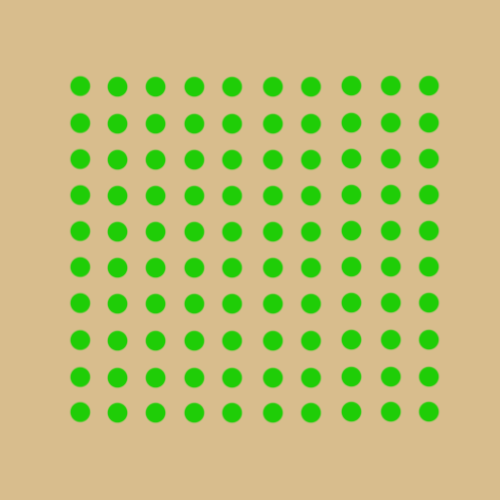
\includegraphics[scale=0.76]{fig/Grid.png}
  \label{fig:grid}
}
\quad 
\subfigure[Final Image with Centroiding]{
  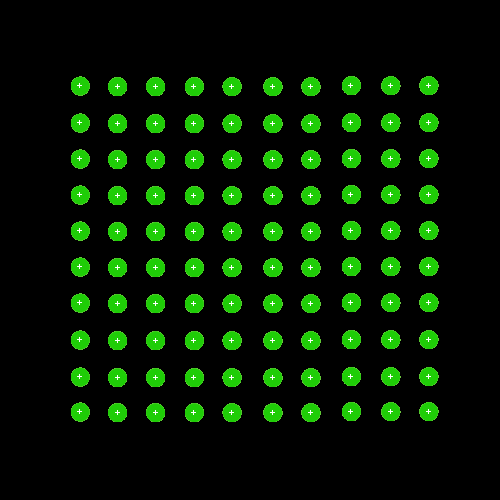
\includegraphics[scale=0.38]{fig/GridCentroiding.png}
  \label{fig:gridCentroiding}
}
\caption{RGB images of a grid of 10 x 10 green points without any noise} 
\end{figure}

In a real application, the grid will not be as perfect as previously after the projection on the rock. Small light spots could be detected as false positive, two points could be slightly linked or some spots could be displaced. In order to deal with these issues, three solutions are implemented: 
\begin{itemize}
\item During the separation step, if a point has an insignificant number of pixel, it is dismissed. The threshold can be adjusted knowing the expected size of a point. 
\item Morphological operations (see Theory Section) such as openings are used to disconnect two linked points. The number of erosion and dilation to carry out to separate the points without loosing too much information about the points have to be calibrated. 
\item A sort algorithm is implemented to obtain the centroids of the beam spots from left to right and from the top to the bottom. It is assumed that all the points projected are detected by the color detection algorithm. Otherwise, without pattern other than an unicolor grid, it is not feasible to know which points have disappeared. As we have a 10x10 grid, the algorithm is looking for the ten centroids of the beam spots which are the most close to the top of the image. They constitute a new row of the sorted table of centroids, being classified by increasing horizontal position. These centroids are then removed from the original table and these steps are reiterated until the ten sorted rows of the grid are added to the sorted table.
\end{itemize}

These techniques are tested on the same grid as above, adding some noise (see figures \ref{fig:noisyGrid} and \ref{fig:noisyGridCentroiding}. To choose the adapted number of erosion and dilation to effectuate the opening, the size of the points have to be taken into account. Indeed, if too many erosions are carried out, all the beam spots will be removed. On the contrary, if not enough are accomplished, two linked spots will not be separated. Each point of the grid is composed of around 300 pixels.  As we want to keep enough pixels to compute an accurate centroid, it is needed to keep at least 50 pixels. Four erosions allow to reach this result, followed by the same number of dilation to retrieve nearly the original number of pixels and to accomplish the opening. To make sure that the opening will only slightly change the centre of mass of the points, the centroiding method was performed on figure \ref{fig:grid} with and without opening. The coordinates of the centroids were exactly the same in the two cases. The opening has preserved the information. It will be assumed that even if there is a slight centroiding error after the opening, it is insignificant.

Several types of noise are added and are denoted figure \ref{fig:noisyGrid}. 
\begin{itemize}
\item The first one shows that small changes of green color on a point or inside the same point do not affect the color detection, but could have an impact on the centroid as it is weighted by the intensity of the color. This kind of noise may appear if the albedo of the target is not uniform for instance.
\item The second noise is a spot of a green-brown color. As it is expected, it is not detected by the color detection algorithm. It may happen, as for the third and fifth noises, if the target contains green minerals for example.
\item The same spot (3 on the figure) but with a color close to the grid points is added to the image. It is detected as a point but its size is under the threshold chosen and it is dismissed as it can be seen on the figure \ref{fig:noisyGridCentroiding}. The opening also ensures that the unexpected spot disappears. 
\item The fourth noise represents two linked points. Thanks to the opening, which reduces the size of the beam spots before increasing them but not as much as they were originally, the connected points are well separated on the final image. This noise can happen if the relief of the target is abrupt.
\item In 5, a smaller green spot (which is noise) is linked to a real point. The spot is tiny and even if it is detected by the color algorithm, the opening is efficient enough to delete it as it is on the edge of a bigger beam spot.
\item Finally, the last kind of perturbation tests if the sort algorithm is effective. Indeed, the point (6) is shifted upward and as the program looks for the green spots row by row, its centroid should be in first position in the second row of the table. Thanks to the sort algorithm, we can notice (by checking the table) that it is not the case and that it is displaced to the right box. This kind slide of the dots will happen each time because the target will not be plane.
\end{itemize}

\begin{figure}[!h] 
\centering
\subfigure[Original Image]{
  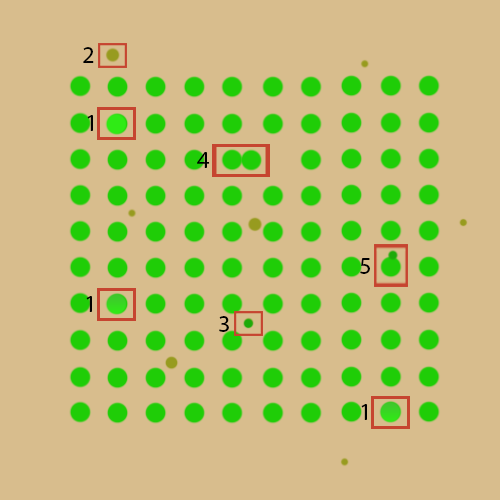
\includegraphics[scale=0.76]{fig/NoisyGrid.png}
  \label{fig:noisyGrid}
}
\quad 
\subfigure[Final Image with Centroiding]{
  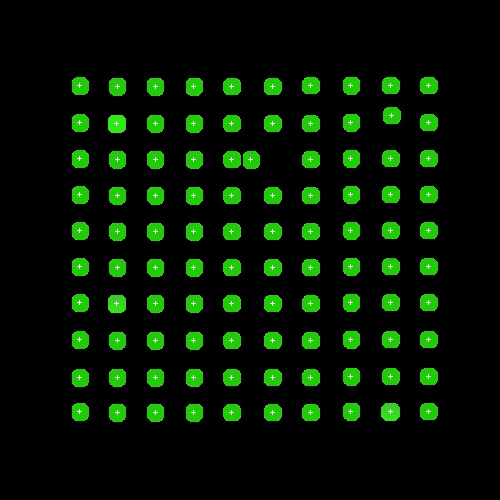
\includegraphics[scale=0.38]{fig/NoisyGridCentroiding.jpg}
  \label{fig:noisyGridCentroiding}
}
\caption{RGB images of a grid of 10 x 10 green points with noise} 
\end{figure}

It can be concluded that the algorithm is robust enough to handle some noise on computed images. Nevertheless, the deformation and the unexpected light spots or reflets on the rocks could be worse than expected and the algorithm may be incapable of finding the cendroid of each point, with no false positive or false negative. To ensure the robustness of the algorithm, integration tests with a real system have to be carried out.